\chapter{Prototype} \label{ch:prototype}

\begin{figure}[H]
    \centering
    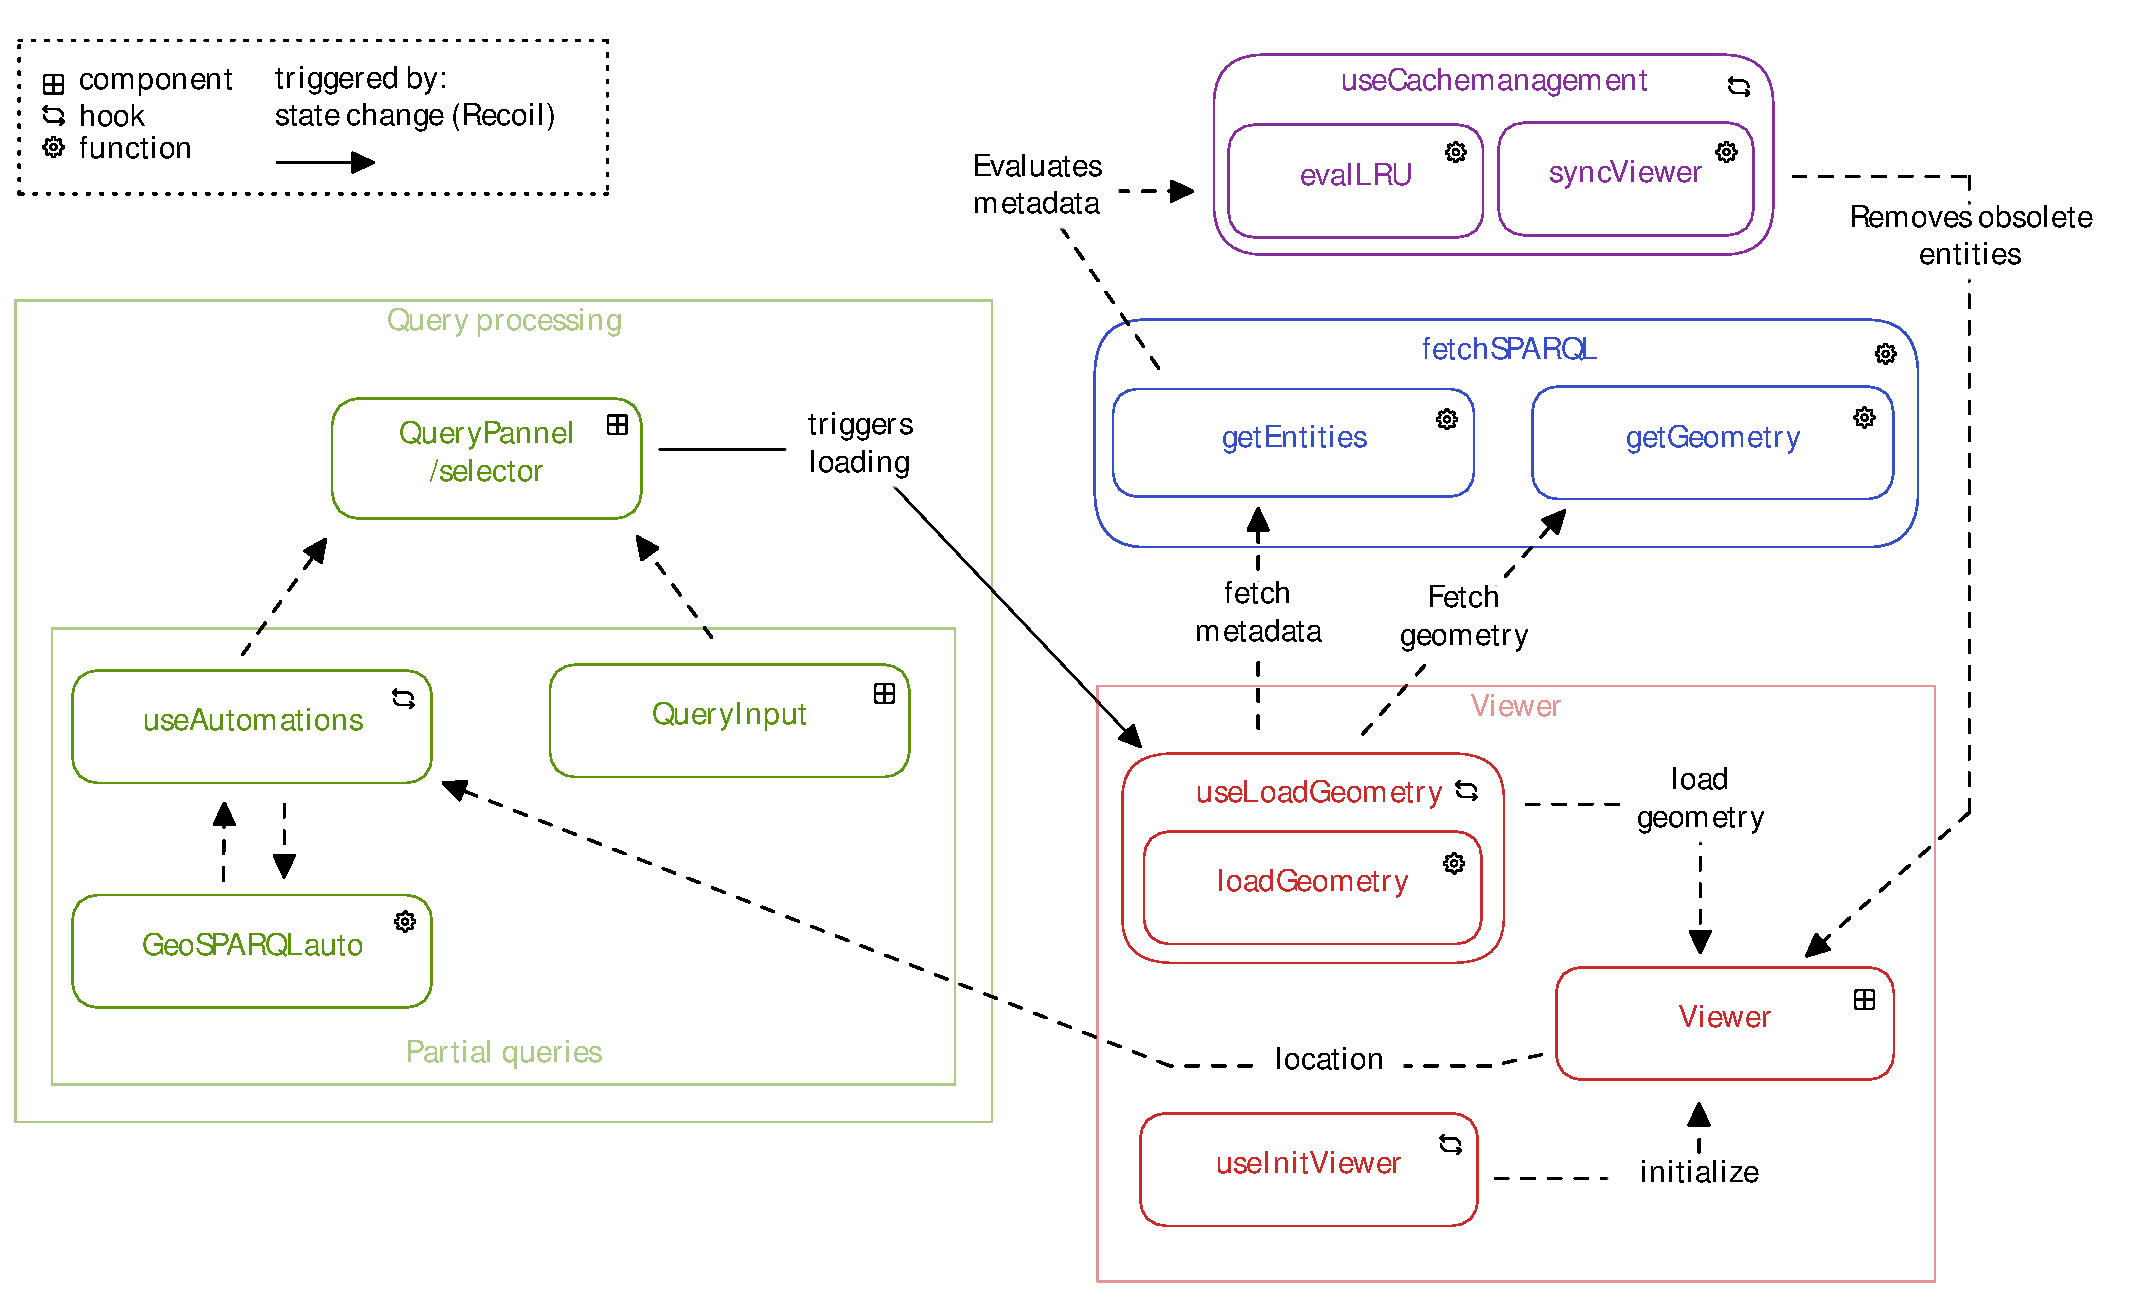
\includegraphics[width=\textwidth]{figures/pdf/interactions_prototype.pdf}
    \caption[Interactions prototype]{Conceptual diagram of the interactions between the moduwithin the prototype, based on Figure \ref{fig:interactionModules}.}
    \label{fig:interactionPrototype}
\end{figure}

\section{Database design}

\section{Web Development Stack}
% describe specific technologies/ Modern Web Development Tools used
\subsection{Next.js}
% why
% react based
% server side rendering
% easy deploy to vercel

\subsection{Recoil}
% why
% state management importance in such app

\subsection{lru\_map}
% npm package by Rasmus Andersson from https://github.com/rsms/js-lru
% advantage of lru without list shifting
% => why used

\subsection{fetch-sparql-endpoint}
% npm package by Ruben Taelman from 
% a Web postdoctoral researcher at IDLab, Ghent University – imec, Belgium
% https://github.com/rubensworks/fetch-sparql-endpoint.js
% https://www.rubensworks.net/


\subsection{Xeokit-\acs{sdk}}

\subsection{\acs{ui} tools}
% importance of visual design

\subsubsection{Tailwindcss}
\subsubsection{Radix}
%% mentioned for use of icon library
\subsubsection{Material UI}
